$y=\ln x$ desde $x=1$ a $x=2\sqrt{2}$.

\nopagebreak
\begin{align*}
y' = 1/x. \quad 1+(y')^2 = 1 + 1/x^2 = \frac{x^2+1}{x^2}. \\
L &= \int_{1}^{2\sqrt{2}} \frac{\sqrt{x^2+1}}{x} \, dx \\
\text{Integral estándar: } \sqrt{x^2+1} - \ln\left(\frac{1+\sqrt{x^2+1}}{x}\right). \\
\text{Evaluando en } 2\sqrt{2}: \sqrt{9} - \ln(\frac{1+3}{2\sqrt{2}}) = 3 - \ln(\sqrt{2}). \\
\text{Evaluando en } 1: \sqrt{2} - \ln(\frac{1+\sqrt{2}}{1}) = \sqrt{2} - \ln(1+\sqrt{2}). \\
L &= 3 - \sqrt{2} + \ln(1+\sqrt{2}) - \ln(\sqrt{2})
\end{align*}

\[
\boxed{\displaystyle 3 - \sqrt{2} + \ln\left(\frac{1+\sqrt{2}}{\sqrt{2}}\right)}
\]

\begin{center}
    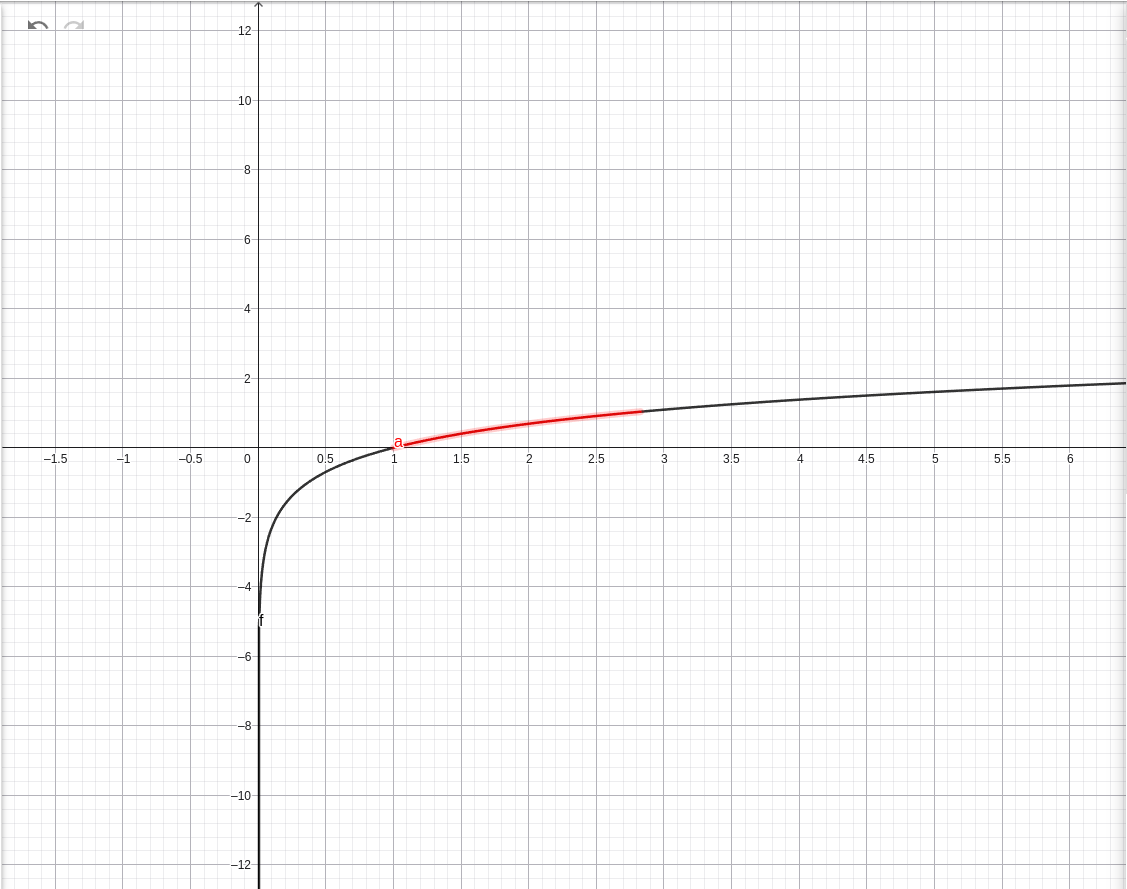
\includegraphics[width=0.5\textwidth]{Graficas/ejer47.png}
\end{center}
